\subsection{Progettazione Concettuale (Modello ER)}

\begin{itemize}
    \item \textbf{input}: specifica informale dei dati
    \item \textbf{output}: schema concettuale indipendente da ogni considerazione implementativa
    \item \textbf{obiettivo primario}: rappresentazione non ambigua deidati
\end{itemize}

\begin{figure}[h]
    \centering
    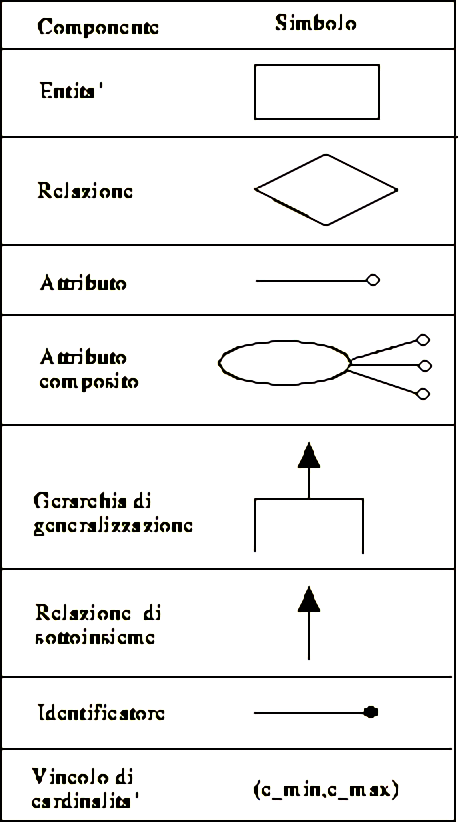
\includegraphics[width=0.5\textwidth, height=4in, keepaspectratio]{images/ER1.png}
    \label{fig:er}
\end{figure}

\subsubsection{Gerarchie}
Data una generalizzazione di $E$ in $E_1, ..., E_n$\\
Possono essere:
\begin{itemize}
    \item \textbf{Totale}: Ogni istanza di $E$ \`e istanza di almeno Un'Entità $E_i$
    \item \textbf{Parziale}: Esiste almeno un'istanza di E che non \`e istanza di alcuna entità $E_i$
\end{itemize}
E
\begin{itemize}
    \item \textbf{Esclusiva}: Ogni istanza di $E$ \`e istanza di al più un'entità $E_i$
    \item \textbf{Condivisa}: Esiste almeno un'istanza di $E$ che \`e istanza di più di un'entità $E_i$
\end{itemize}

\subsection{Ristrutturazione}
\subsubsection{Partizionamento/Accorpamento di entità}
Se ci sono operazioni frequenti che coinvolgono solo un sottoinsieme degli attributi di E si \textbf{partiziona} l'entità a seconda di tali attributi.\\
Se invece ci sono operazioni frequenti che riguardano due entità, si \textbf{accorpano}. Quest'ultima operazione può generare attributi opzionali in alcuni casi.\\
Questa operazione viene più spesso eseguita nella fase di \textbf{Progettazione Logica}.

\subsubsection{Eliminazione degli attributi composti}
\begin{itemize}
    \item \textbf{Soluzione 1}: merge dei sotto-attributi di A in un unico attributo semplice
    \begin{itemize}
        \item diventa responsabilità delle applicazioni garantire che il nuovo attributo contenga valori coerenti con la semantica dell'attributo composto ristrutturato.
        \item fare merge e unmerge
    \end{itemize}
    \item \textbf{Soluzione 2}: considerare tutti i sotto-attributi di A come attributi di E
    \begin{itemize}
        \item ridefinizione del dominio dell'attributo
        \item si perde la relazione tra i sotto-attributi
    \end{itemize}
    \item \textbf{Soluzione 3}: introdurre un’entità per rappresentare il tipo di A e associarla ad E
\end{itemize}

\subsubsection{Eliminazione degli attributi multi-valore}
Data un’entità $E$ con un attributo multi-valore $A$:
\begin{itemize}
    \item si definisce una nuova entità $E_A$ con un attributo mono-valore $A$
    \item si collegano $E$ ed $E_A$ tramite un'associazione $R_A$
\end{itemize}

\subsubsection{Eliminazione delle gerarchie di generalizzazione}
Entità $E$ generalizzazione di entità $E_1,...,E_n$. A seconda del tipo di gerarchia e del carico di lavoro si sceglie una delle seguenti soluzioni:
\begin{itemize}
    \item Eliminazione entità figlie
    \item Eliminazione entità padre
    \item Sostituzione della generalizzazione con associazioni
\end{itemize}
\newpage \noindent
\textbf{Eliminazione entità figlie}
\begin{itemize}
    \item Entità
    \begin{itemize}
        \item $E_1,...,E_n$ vengono eliminate
    \end{itemize}
    
    \item Attributi
    \begin{itemize}
        \item gli attributi di $E_1,...,E_n$ loro attributi vengono inseriti in $E$ come opzionali
        
        \item si aggiunge ad $E$ un attributo tipo che specifica da quale entità figlia $E_i$ proviene l’istanza dell'entità padre nello schema ristrutturato
        \begin{itemize}
            \item nel caso di generalizzazioni totali, non può mai essere nullo
            \item nel caso di generalizzazioni parziali, un valore nullo indica un'istanza di $E$ che, nello schema originario, non era istanza di nessuna $E_i$
            \item nel caso di generalizzazioni condivise, sarà multi-valore
        \end{itemize}
        
        \item bisogna aggiungere un vincolo di integrità per garantire che se tipo $= E_i$, gli attributi obbligatori di $E_i$ siano non nulli
        
        \item bisogna aggiungere un vincolo di integrità per garantire che se un
        attributo di $E_i$ è non nullo, allora tipo = $E_i$ (se la generalizzazione è
        condivisa, $E_i$ è uno dei valori assunti da tipo)
    \end{itemize}
    
    \item Associazioni
    \begin{itemize}
        \item La partecipazione (obbligatoria od opzionale) di un'entità figlia ad un'associazione diventa la partecipazione opzionale dell'entità padre alla stessa associazione
        \item Per ogni associazione, bisogna aggiungere un vincolo di integrità che indichi quali tipi di istanze dell'entità padre possono essere coinvolti nell'associazione
    \end{itemize}
\end{itemize}
\vspace{2mm} \noindent
\textbf{Eliminazione entità padre}
\begin{itemize}
    \item Applicabile solo nel caso di generalizzazione totale
    
    \item Entità
    \begin{itemize}
        \item eliminazione dell'entità padre $E$
    \end{itemize}
    
    \item Attributi
    \begin{itemize}
        \item inserimento degli attributi di $E$ in ciascuna delle entità figlie
    \end{itemize}

    \item Associazioni
    \begin{itemize}
        \item ogni associazione a cui partecipava $E$ viene sostituita con $n$ nuove associazioni, una per ogni $E_i$
    \end{itemize}

    \item Vincoli di integrità
    \begin{itemize}
        \item se la generalizzazione esclusiva, vincolo per indicare che, nello schema ristrutturato, non possono esistere istanze di due entità figlie distinte aventi lo stesso valore per gli identificatori (ereditati dall'entità padre)
        \item il vincolo di cardinalità di ciascuna entità figlia rispetto alla nuova associazione coinciderà con il vincolo di cardinalità dell'entità padre rispetto all'associazione eliminata
        \item i vincoli di cardinalità delle altre entità diventeranno invece opzionali
    \end{itemize}
\end{itemize}
\newpage \noindent
\textbf{Sostituzione della generalizzazione con associazioni}
\begin{itemize}
    \item Entità
    \begin{itemize}
        \item non modificate
    \end{itemize}
    
    \item Associazioni
    \begin{itemize}
        \item la gerarchia viene sostituita da n associazioni $R_i$ uno a uno, che collegano $E$ con $E_i$
        \item ciascun $E_i$ è identificata esternamente da $E$ e partecipa obbligatoriamente a $R_i$
        \item la partecipazione di $E$ a ciascun $R_i$ è opzionale
    \end{itemize}
    
    \item Vincoli di integrità
    \begin{itemize}
        \item se la generalizzazione è esclusiva, un'istanza di $E$ non può partecipare contemporaneamente a due o più associazioni $R_i$
        \item se la generalizzazione è totale, ogni istanza di $E$ deve partecipare obbligatoriamente ad almeno un’associazione $R_i$
    \end{itemize}
\end{itemize}

\subsection{Traduzione}
Porta dallo schema concettuale ristrutturato allo schema logico
$$\text{Entità} \Rightarrow \text{Relazione}$$
$$\text{Associazione} \Rightarrow \text{Relazione o Chiave esterna}$$

\subsubsection{Traduzione associazione binaria molti a molti}
L’associazione diventa una relazione indipendente con Attributi:
\begin{itemize}
    \item chiavi delle entità coinvolte
    \item come chiavi esterne verso le relazioni che rappresentano le entità
    \item quelli propri dell'associazione
\end{itemize}

\subsubsection{Traduzione associazione n-aria molti a molti}
Molto spesso analogo ad associazioni binarie.

\subsubsection{Traduzione associazione binaria uno a *}
Si può o generare una relazione con due chiavi esterne (e una chiave) o accorpare l'entità dando quindi a una delle Relazioni la chiave esterna ed eventuali attributi dell'associazione.

\subsubsection{Traduzione associazione binaria uno a uno}
Se entrambe partecipano univocamente ((1, 1), (1, 1)) si può scegliere con quale accorpare l’associazione sulla base del carico di lavoro.\\
Altrimenti se sono opzionali ((0, 1), (0, 1)) si usano valori opzionali se si accorpano o, in alternativa, si crea una Relazione corrispondente all'associazione come per uno a *.

\subsubsection{Traduzione associazione n-aria uno a molti}
Si accorpa ad una Relazione tutte le chiavi delle altre ed eventuali attributi della associazione.

\subsection{Progettazione Logica}
\begin{itemize}
    \item \textbf{input}: schema concettuale dei dati + informazioni sul carico atteso (+ scelta del DBMS)
    \item \textbf{output}: schema logico per il DBMS prescelto equivalente allo schema concettuale ottimizzato per (lo specifico DBMS) e l’uso atteso
    \item \textbf{obiettivo primario}: rappresentazione dei dati focalizzata alla realizzazione della base di dati e delle relative applicazioni
\end{itemize}
\noindent
Produce uno schema logico del tipo:
\begin{center}
    Tabella(\underline{chiavi}, \textit{chiavi secondarie}, $\text{chiavi esterne}^{\text{Tabella riferita}}$, attributi normali)\\
    ...
\end{center}

\subsection{Normalizzazione}
Verifica di qualità dello schema logico prodotto, effettuata tramite opportuni strumenti formali.

\subsection{Progettazione Fisica}
In questa fase vengono effettuate alcune scelte circa la memorizzazione fisica dei dati (ad esempio, indici)